%
% Clonedel.tex
%
% History of LulzBot Printers
%
% Copyright (C) 2014, 2015 Aleph Objects, Inc.
%
% This document is licensed under the Creative Commons Attribution 4.0
% International Public License (CC BY-SA 4.0) by Aleph Objects, Inc.
%

\begin{figure}[h!]
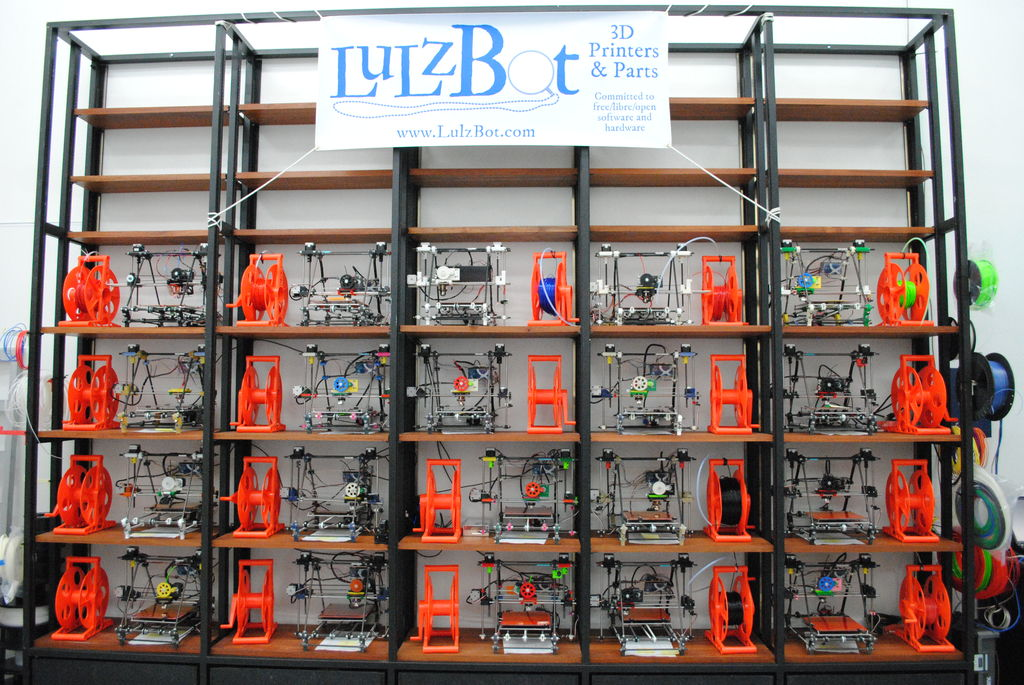
\includegraphics[keepaspectratio=true,height=0.40\textheight,width=1.00\textwidth,angle=0]{clonedel/clonedel-display.jpg}
 \caption{LulzBot Clonedels.}
 \label{fig:clonedel-clonedel-display}
\end{figure}

LulzBot Clonedels were made from silicon molds purchased (PO00077)
from Metrix Createspace on February 23, 2011. Eleven or more units were made,
starting with ``Mars P4''. The Clonedels printed the subsequent LulzBot Prusas.
Units through ``P64'' had some Clonedel parts.

%
% LulzBot Clonedel.tex
%
% History of LulzBot Printers
%
% Copyright (C) 2014, 2015 Aleph Objects, Inc.
%
% This document is licensed under the Creative Commons Attribution 4.0
% International Public License (CC BY-SA 4.0) by Aleph Objects, Inc.
%

\section{LulzBot Clonedel Molds}
The LulzBot Clonedel parts themselves were primarily poured from silicon molds.

\begin{figure}[h!]
\thisfloatpagestyle{empty}
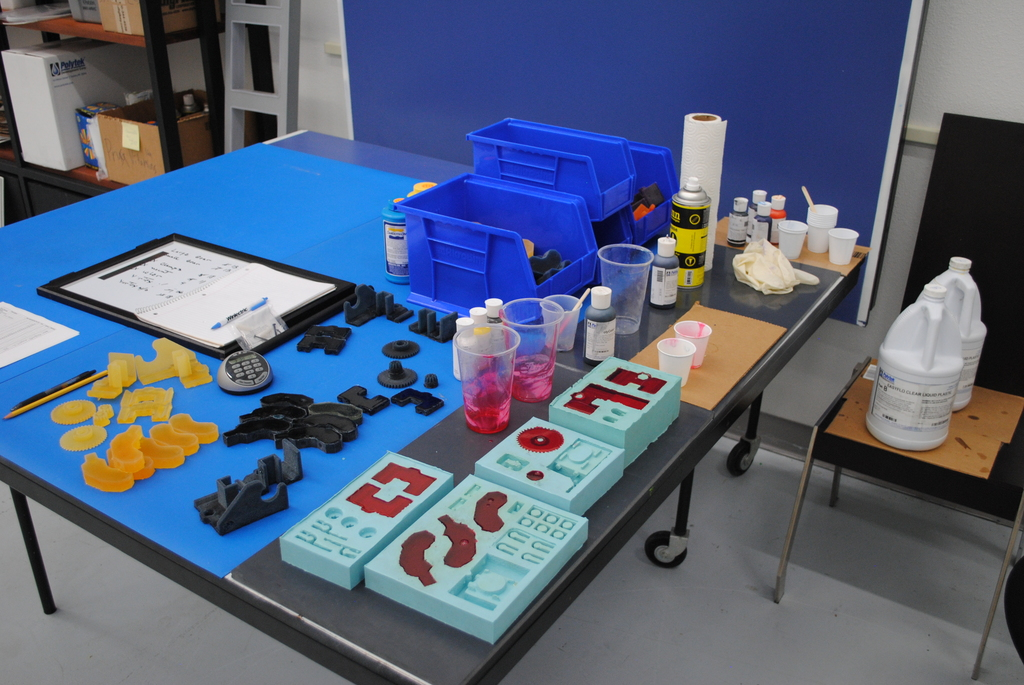
\includegraphics[keepaspectratio=true,height=0.40\textheight,width=1.00\textwidth,angle=0]{clonedel/table-layout.jpg}
 \caption{LulzBot Clonedel production ping pong table.}
 \label{fig:clonedel-table-layout}
\end{figure}

\begin{figure}[h!]
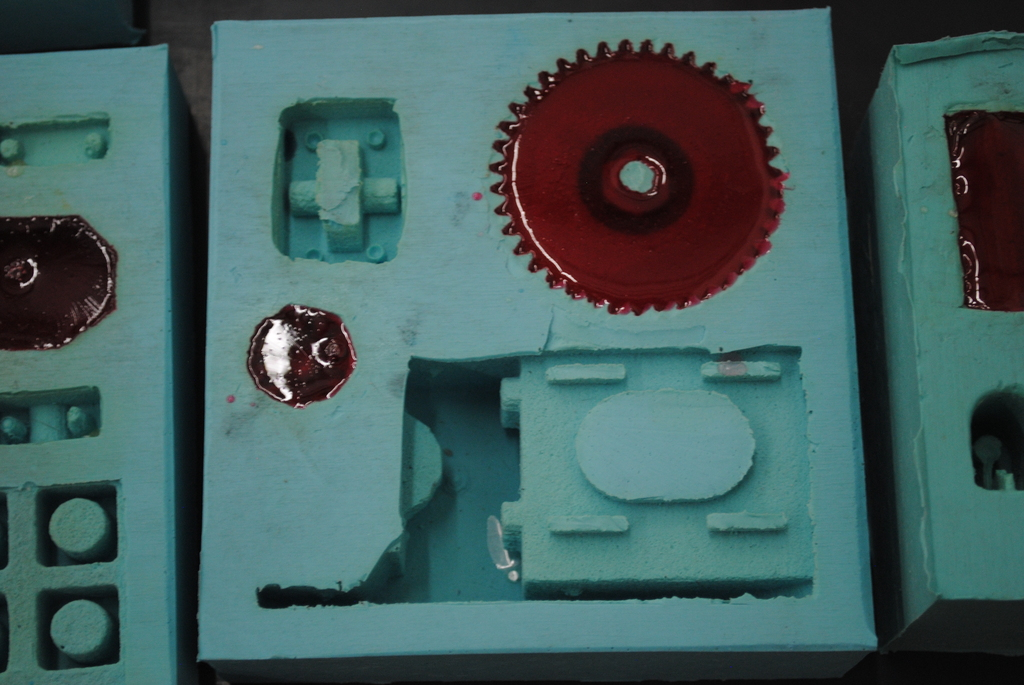
\includegraphics[keepaspectratio=true,height=0.40\textheight,width=1.00\textwidth,angle=0]{clonedel/gear-pour.jpg}
 \caption{LulzBot Clonedel gears in the silicon mold.}
 \label{fig:clonedel-gear-pour}
\end{figure}

\begin{figure}[h!]
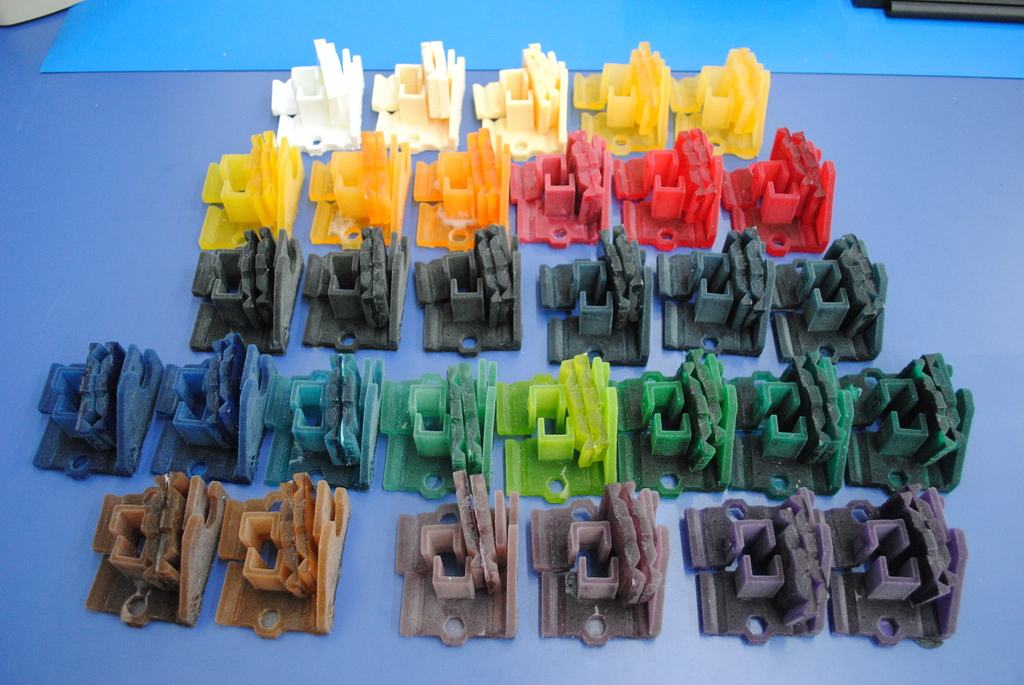
\includegraphics[keepaspectratio=true,height=0.40\textheight,width=1.00\textwidth,angle=0]{clonedel/clamps.jpg}
 \caption{LulzBot Clonedel molded parts.}
 \label{fig:clonedel-clamps}
\end{figure}

\begin{figure}[h!]
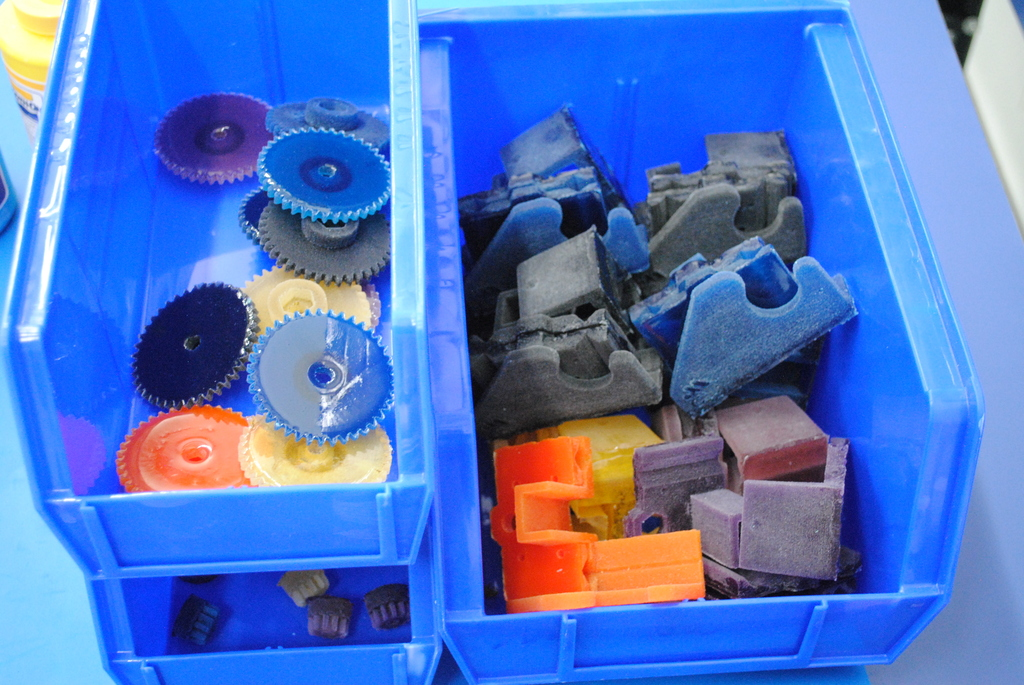
\includegraphics[keepaspectratio=true,height=0.40\textheight,width=1.00\textwidth,angle=0]{clonedel/gears-parts.jpg}
 \caption{LulzBot Clonedel molded gears.}
 \label{fig:clonedel-gears-parts}
\end{figure}


%
% Clonedel.tex
%
% History of LulzBot Printers
%
% Copyright (C) 2014, 2015 Aleph Objects, Inc.
%
% This document is licensed under the Creative Commons Attribution 4.0
% International Public License (CC BY-SA 4.0) by Aleph Objects, Inc.
%

\section{LulzBot Clonedel Mars P4}
LulzBot Clonedel Mars P4.

\begin{figure}[h!]
\thisfloatpagestyle{empty}
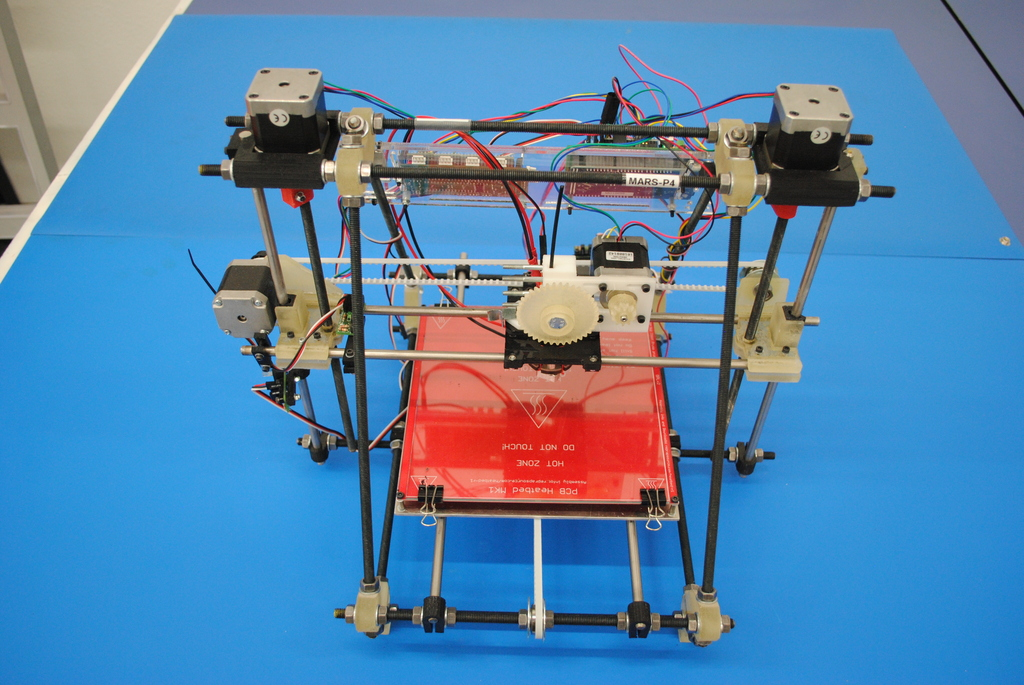
\includegraphics[keepaspectratio=true,height=0.40\textheight,width=1.00\textwidth,angle=0]{clonedel/mars-p4-front.jpg}
 \caption{LulzBot Clonedel Mars P4 Front}
 \label{fig:clonedel-mars-p4-front}
\end{figure}

\begin{figure}[h!]
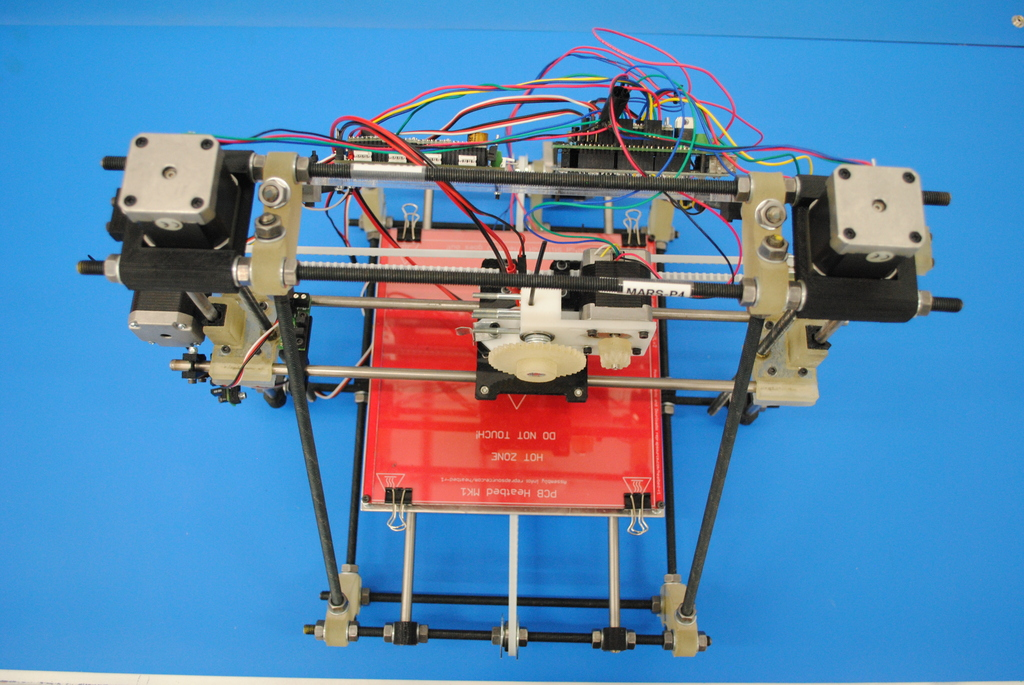
\includegraphics[keepaspectratio=true,height=0.40\textheight,width=1.00\textwidth,angle=0]{clonedel/mars-p4-top.jpg}
 \caption{LulzBot Clonedel Mars P4 Top}
 \label{fig:clonedel-mars-p4-top}
\end{figure}

\begin{figure}[h!]
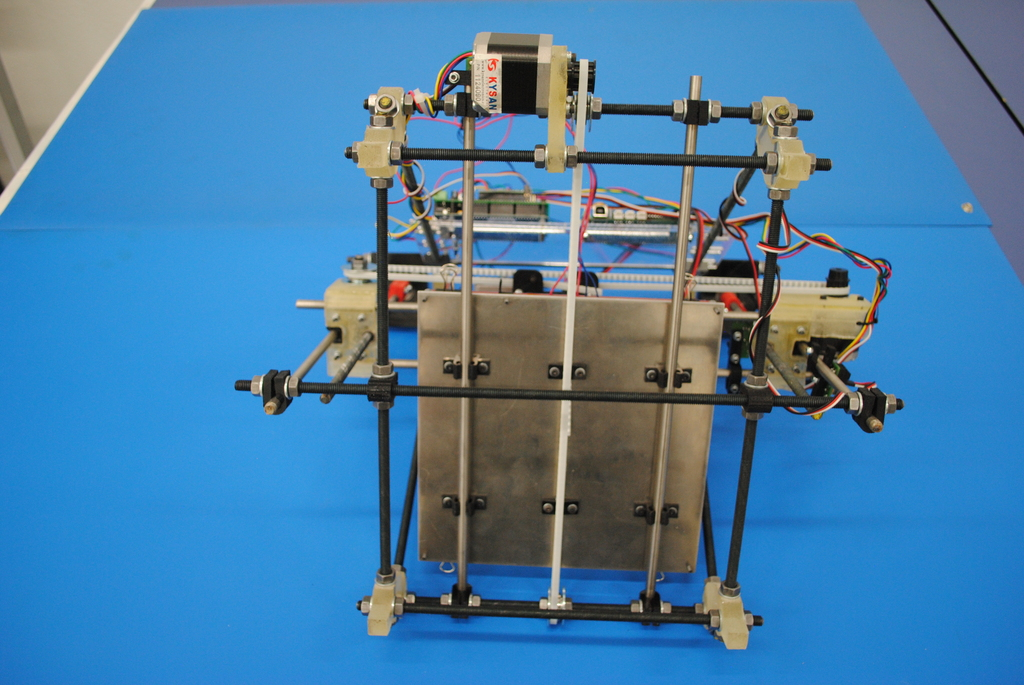
\includegraphics[keepaspectratio=true,height=0.40\textheight,width=1.00\textwidth,angle=0]{clonedel/mars-p4-bottom.jpg}
 \caption{LulzBot Clonedel Mars P4 Bottom}
 \label{fig:clonedel-mars-p4-bottom}
\end{figure}

\begin{figure}[h!]
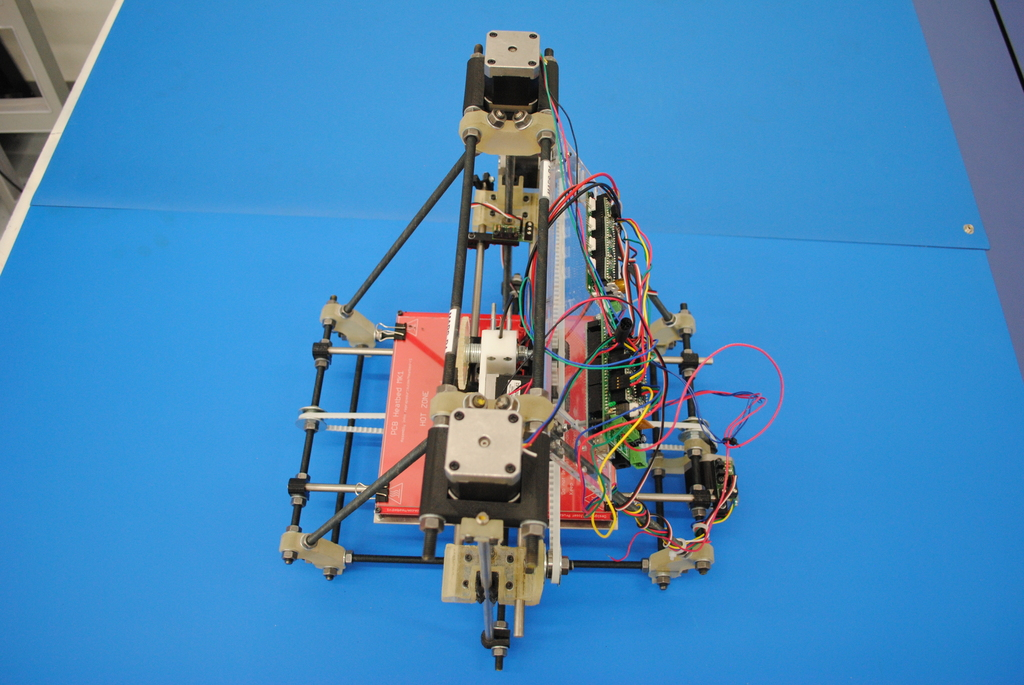
\includegraphics[keepaspectratio=true,height=0.40\textheight,width=1.00\textwidth,angle=0]{clonedel/mars-p4-top-right.jpg}
 \caption{LulzBot Clonedel Mars P4 Top Right}
 \label{fig:clonedel-mars-p4-top-right}
\end{figure}

\begin{figure}[h!]
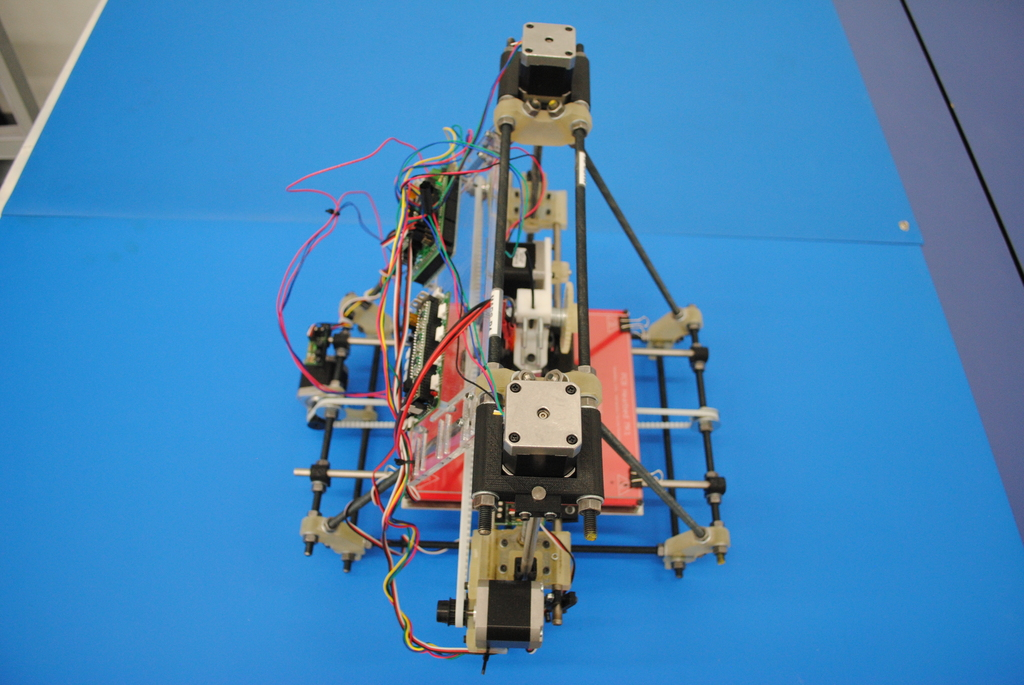
\includegraphics[keepaspectratio=true,height=0.40\textheight,width=1.00\textwidth,angle=0]{clonedel/mars-p4-top-left.jpg}
 \caption{LulzBot Clonedel Mars P4 Top Left}
 \label{fig:clonedel-mars-p4-top-left}
\end{figure}


%
% Clonedel.tex
%
% History of LulzBot Printers
%
% Copyright (C) 2014, 2015 Aleph Objects, Inc.
%
% This document is licensed under the Creative Commons Attribution 4.0
% International Public License (CC BY-SA 4.0) by Aleph Objects, Inc.
%

\section{LulzBot Clonedel Mars P5}
LulzBot Clonedel Mars P5.

\begin{figure}[h!]
\thisfloatpagestyle{empty}
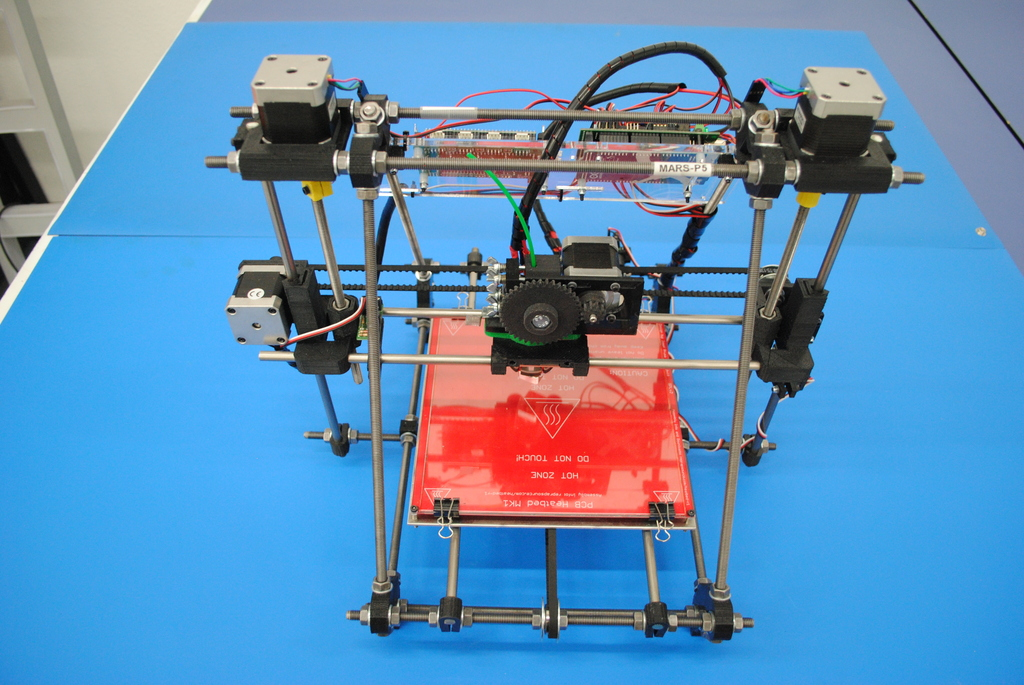
\includegraphics[keepaspectratio=true,height=0.40\textheight,width=1.00\textwidth,angle=0]{clonedel/mars-p5-front.jpg}
 \caption{LulzBot Clonedel Mars P5 Front}
 \label{fig:clonedel-mars-p5-front}
\end{figure}

%clonedel/mars-p5-bottom.jpg
%clonedel/mars-p5-front.jpg
%clonedel/mars-p5-top.jpg
%clonedel/mars-p5-top-left.jpg
%clonedel/mars-p5-top-right.jpg


%
% Clonedel.tex
%
% History of LulzBot Printers
%
% Copyright (C) 2014, 2015 Aleph Objects, Inc.
%
% This document is licensed under the Creative Commons Attribution 4.0
% International Public License (CC BY-SA 4.0) by Aleph Objects, Inc.
%

\section{LulzBot Clonedel Mars P6}
LulzBot Clonedel Mars P6.

\begin{figure}[h!]
\thisfloatpagestyle{empty}
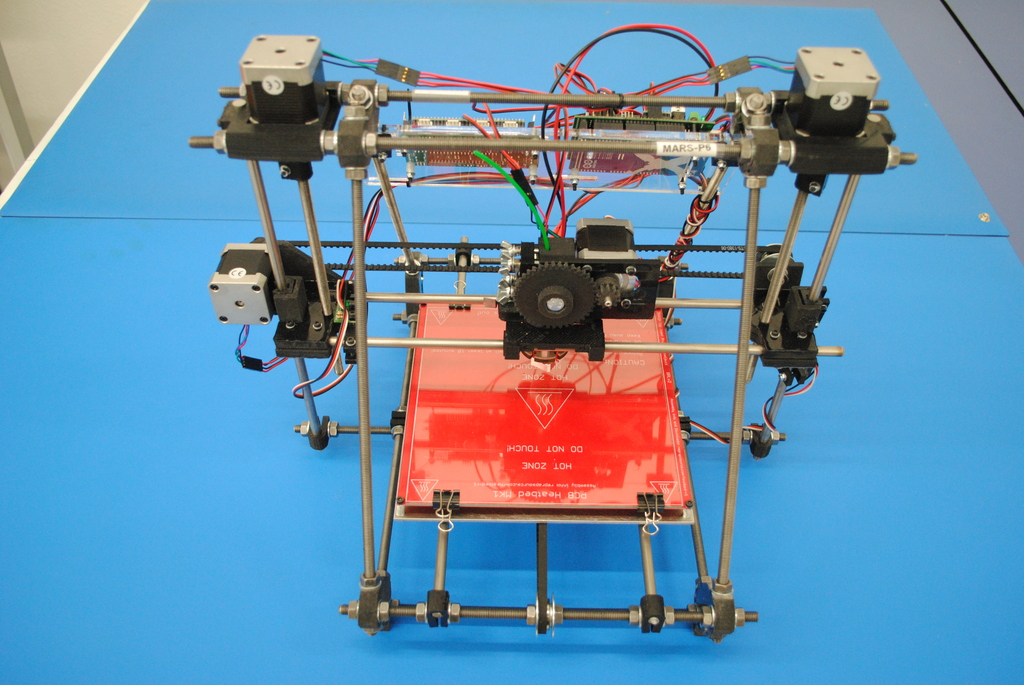
\includegraphics[keepaspectratio=true,height=0.40\textheight,width=1.00\textwidth,angle=0]{clonedel/mars-p6-front.jpg}
 \caption{LulzBot Clonedel Mars P6 Front}
 \label{fig:clonedel-mars-p6-front}
\end{figure}

%clonedel/mars-p6-bottom.jpg
%clonedel/mars-p6-front.jpg
%clonedel/mars-p6-top.jpg
%clonedel/mars-p6-top-left.jpg
%clonedel/mars-p6-top-right.jpg


%
% Clonedel.tex
%
% History of LulzBot Printers
%
% Copyright (C) 2014, 2015 Aleph Objects, Inc.
%
% This document is licensed under the Creative Commons Attribution 4.0
% International Public License (CC BY-SA 4.0) by Aleph Objects, Inc.
%

\section{LulzBot Clonedel Mars P7}
LulzBot Clonedel Mars P7.

\begin{figure}[h!]
\thisfloatpagestyle{empty}
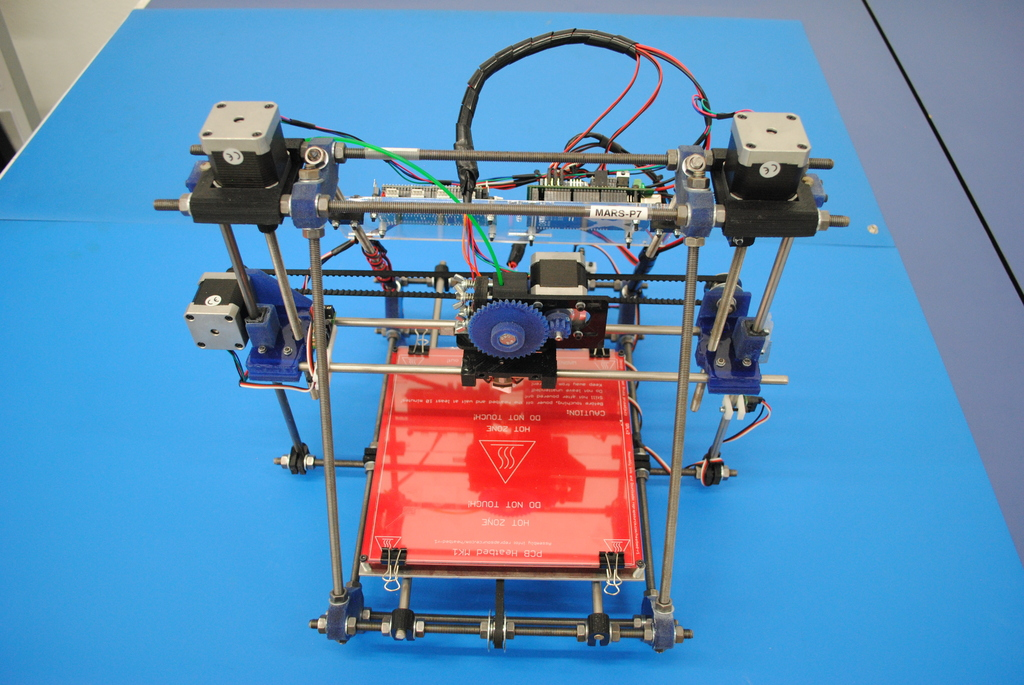
\includegraphics[keepaspectratio=true,height=0.40\textheight,width=1.00\textwidth,angle=0]{clonedel/mars-p7-front.jpg}
 \caption{LulzBot Clonedel Mars P7 Front}
 \label{fig:clonedel-mars-p7-front}
\end{figure}

%clonedel/mars-p7-bottom.jpg
%clonedel/mars-p7-front.jpg
%clonedel/mars-p7-top.jpg
%clonedel/mars-p7-top-left.jpg
%clonedel/mars-p7-top-right.jpg


%
% Clonedel.tex
%
% History of LulzBot Printers
%
% Copyright (C) 2014, 2015 Aleph Objects, Inc.
%
% This document is licensed under the Creative Commons Attribution 4.0
% International Public License (CC BY-SA 4.0) by Aleph Objects, Inc.
%

\section{LulzBot Clonedel Mars P8}
LulzBot Clonedel Mars P8.

\begin{figure}[h!]
\thisfloatpagestyle{empty}
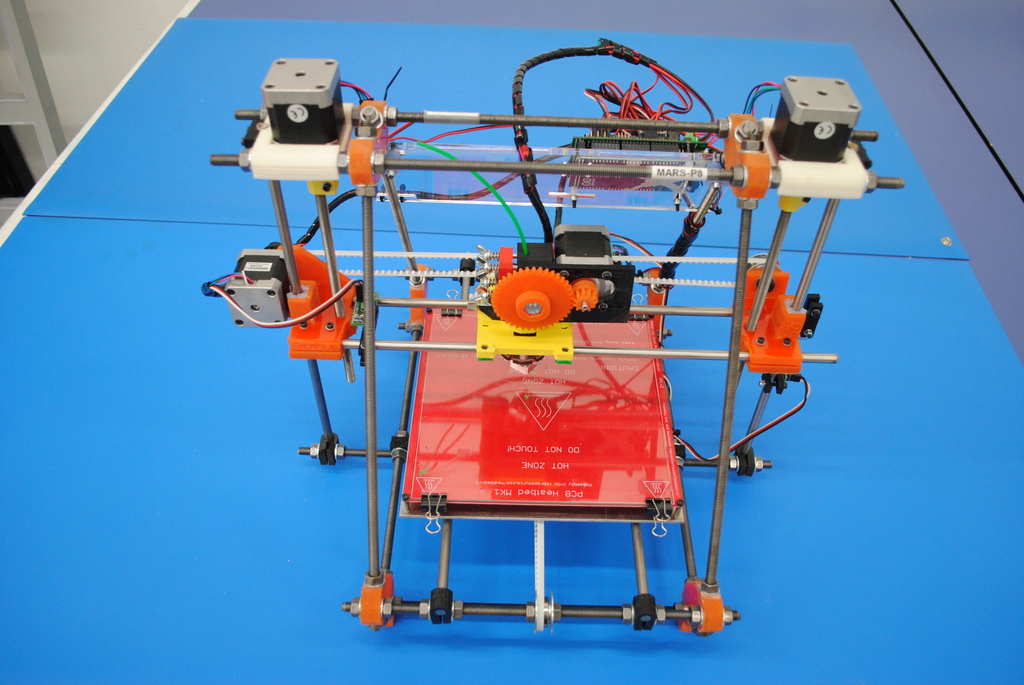
\includegraphics[keepaspectratio=true,height=0.40\textheight,width=1.00\textwidth,angle=0]{clonedel/mars-p8-front.jpg}
 \caption{LulzBot Clonedel Mars P8 Front}
 \label{fig:clonedel-mars-p8-front}
\end{figure}

%clonedel/mars-p8-bottom.jpg
%clonedel/mars-p8-front.jpg
%clonedel/mars-p8-top.jpg
%clonedel/mars-p8-top-left.jpg
%clonedel/mars-p8-top-right.jpg


%
% Clonedel.tex
%
% History of LulzBot Printers
%
% Copyright (C) 2014, 2015 Aleph Objects, Inc.
%
% This document is licensed under the Creative Commons Attribution 4.0
% International Public License (CC BY-SA 4.0) by Aleph Objects, Inc.
%

\section{LulzBot Clonedel Mars P9}
LulzBot Clonedel Mars P9.

\begin{figure}[h!]
\thisfloatpagestyle{empty}
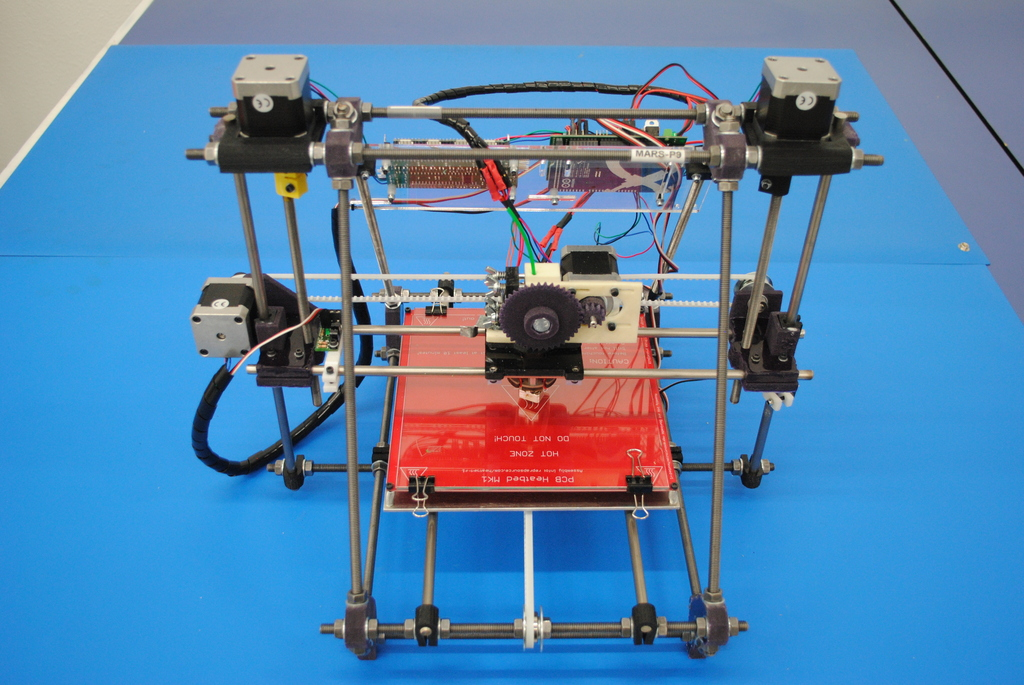
\includegraphics[keepaspectratio=true,height=0.40\textheight,width=1.00\textwidth,angle=0]{clonedel/mars-p9-front.jpg}
 \caption{LulzBot Clonedel Mars P9 Front}
 \label{fig:clonedel-mars-p9-front}
\end{figure}

%clonedel/mars-p9-bottom.jpg
%clonedel/mars-p9-front.jpg
%clonedel/mars-p9-top.jpg
%clonedel/mars-p9-top-left.jpg
%clonedel/mars-p9-top-right.jpg


%
% Clonedel.tex
%
% History of LulzBot Printers
%
% Copyright (C) 2014, 2015 Aleph Objects, Inc.
%
% This document is licensed under the Creative Commons Attribution 4.0
% International Public License (CC BY-SA 4.0) by Aleph Objects, Inc.
%

\section{LulzBot Clonedel Mars P10}
LulzBot Clonedel Mars P10.

\begin{figure}[h!]
\thisfloatpagestyle{empty}
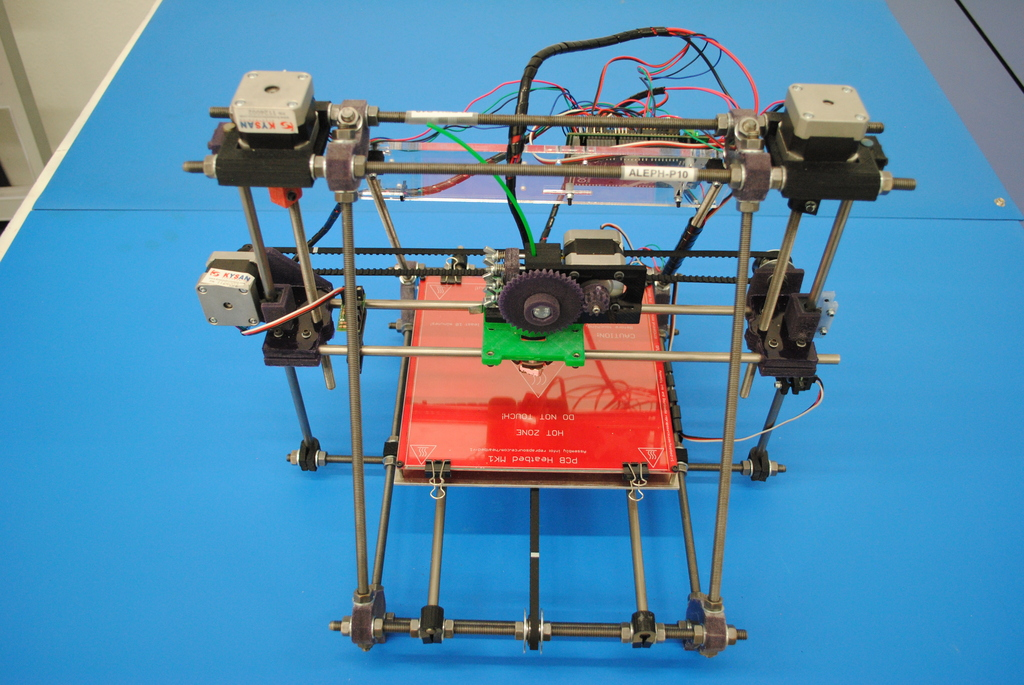
\includegraphics[keepaspectratio=true,height=0.40\textheight,width=1.00\textwidth,angle=0]{clonedel/mars-p10-front.jpg}
 \caption{LulzBot Clonedel Mars P10 Front}
 \label{fig:clonedel-mars-p10-front}
\end{figure}

%clonedel/mars-p10-bottom.jpg
%clonedel/mars-p10-front.jpg
%clonedel/mars-p10-top.jpg
%clonedel/mars-p10-top-left.jpg
%clonedel/mars-p10-top-right.jpg


%
% Clonedel.tex
%
% History of LulzBot Printers
%
% Copyright (C) 2014, 2015 Aleph Objects, Inc.
%
% This document is licensed under the Creative Commons Attribution 4.0
% International Public License (CC BY-SA 4.0) by Aleph Objects, Inc.
%

\section{LulzBot Clonedel Mars P11}
LulzBot Clonedel Mars P11.

\begin{figure}[h!]
\thisfloatpagestyle{empty}
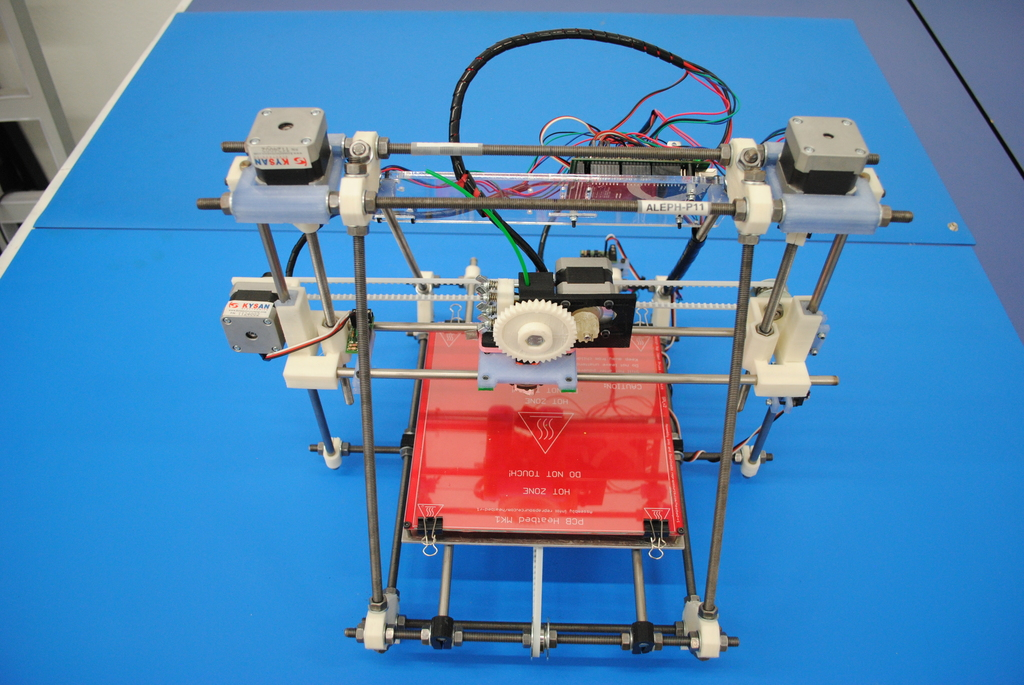
\includegraphics[keepaspectratio=true,height=0.40\textheight,width=1.00\textwidth,angle=0]{clonedel/mars-p11-front.jpg}
 \caption{LulzBot Clonedel Mars P11 Front.}
 \label{fig:clonedel-mars-p11-front}
\end{figure}

%clonedel/mars-p11-bottom.jpg
%clonedel/mars-p11-front.jpg
%clonedel/mars-p11-top.jpg
%clonedel/mars-p11-top-left.jpg
%clonedel/mars-p11-top-right.jpg


%
% Clonedel.tex
%
% History of LulzBot Printers
%
% Copyright (C) 2014, 2015 Aleph Objects, Inc.
%
% This document is licensed under the Creative Commons Attribution 4.0
% International Public License (CC BY-SA 4.0) by Aleph Objects, Inc.
%

\section{LulzBot Clonedel Mars P12}
LulzBot Clonedel Mars P12.

\begin{figure}[h!]
\thisfloatpagestyle{empty}
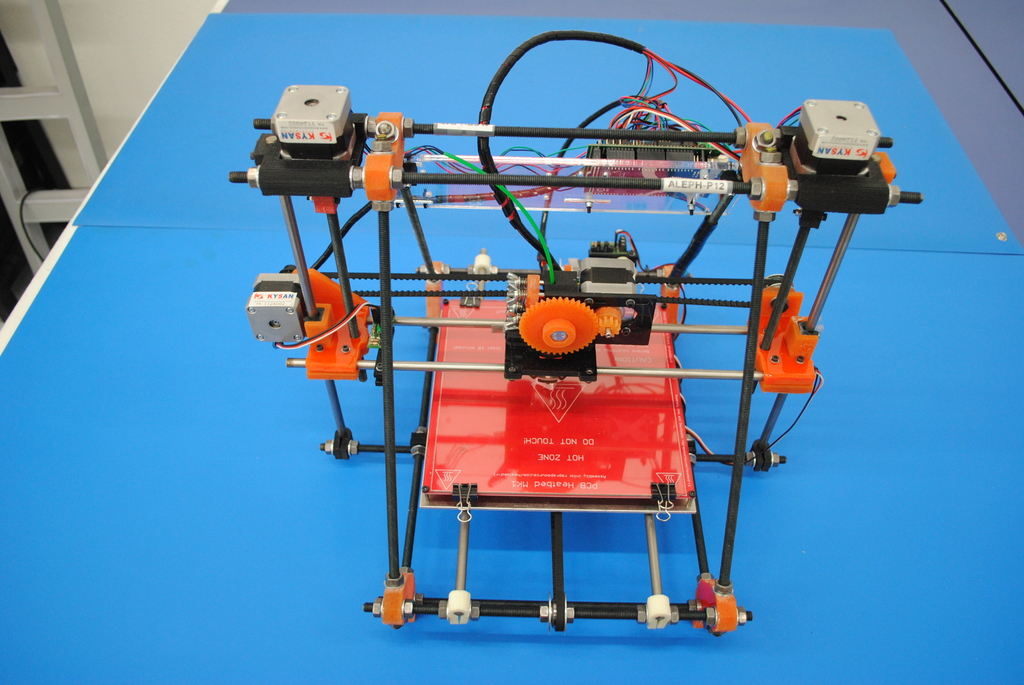
\includegraphics[keepaspectratio=true,height=0.40\textheight,width=1.00\textwidth,angle=0]{clonedel/mars-p12-front.jpg}
 \caption{LulzBot Clonedel Mars P12 Front.}
 \label{fig:clonedel-mars-p12-front}
\end{figure}

%clonedel/mars-p12-bottom.jpg
%clonedel/mars-p12-front.jpg
%clonedel/mars-p12-top.jpg
%clonedel/mars-p12-top-left.jpg
%clonedel/mars-p12-top-right.jpg


%
% Clonedel.tex
%
% History of LulzBot Printers
%
% Copyright (C) 2014, 2015 Aleph Objects, Inc.
%
% This document is licensed under the Creative Commons Attribution 4.0
% International Public License (CC BY-SA 4.0) by Aleph Objects, Inc.
%

\section{LulzBot Clonedel Mars P13}
LulzBot Clonedel Mars P13.

\begin{figure}[h!]
\thisfloatpagestyle{empty}
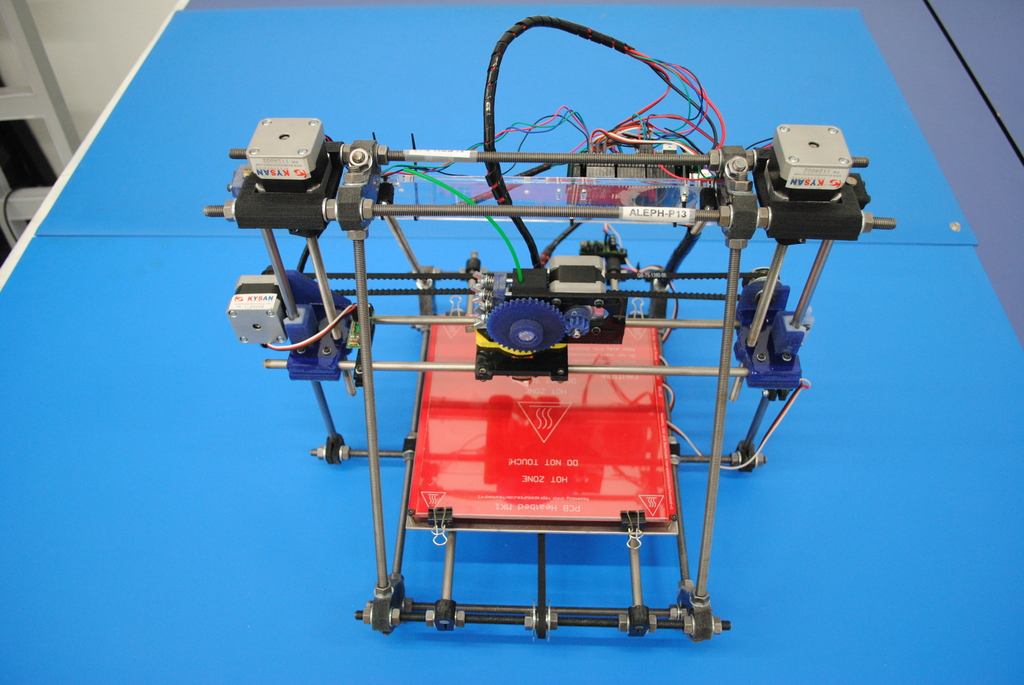
\includegraphics[keepaspectratio=true,height=0.40\textheight,width=1.00\textwidth,angle=0]{clonedel/mars-p13-front.jpg}
 \caption{LulzBot Clonedel Mars P13 Front.}
 \label{fig:clonedel-mars-p13-front}
\end{figure}

%clonedel/mars-p13-bottom.jpg
%clonedel/mars-p13-front.jpg
%clonedel/mars-p13-top.jpg
%clonedel/mars-p13-top-left.jpg
%clonedel/mars-p13-top-right.jpg


%
% Clonedel.tex
%
% History of LulzBot Printers
%
% Copyright (C) 2014, 2015 Aleph Objects, Inc.
%
% This document is licensed under the Creative Commons Attribution 4.0
% International Public License (CC BY-SA 4.0) by Aleph Objects, Inc.
%

\section{LulzBot Clonedel Mars P14}
LulzBot Clonedel Mars P14.

\begin{figure}[h!]
\thisfloatpagestyle{empty}
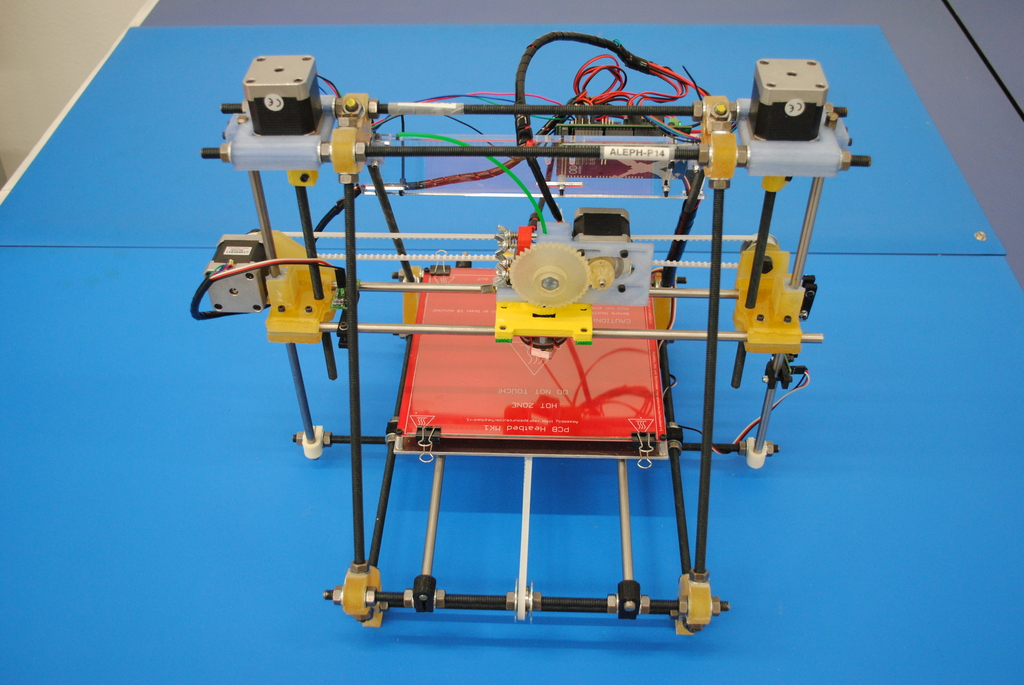
\includegraphics[keepaspectratio=true,height=0.40\textheight,width=1.00\textwidth,angle=0]{clonedel/mars-p14-front.jpg}
 \caption{LulzBot Clonedel Mars P14 Front.}
 \label{fig:clonedel-mars-p14-front}
\end{figure}

%clonedel/mars-p14-bottom.jpg
%clonedel/mars-p14-front.jpg
%clonedel/mars-p14-top.jpg
%clonedel/mars-p14-top-left.jpg
%clonedel/mars-p14-top-right.jpg



